\documentclass{article}

\usepackage{graphicx}
\usepackage{tikz}
\usepackage{tikzsymbols}
\usetikzlibrary{calc,patterns,shapes.geometric}
\pagestyle{empty}
\usepackage[margin=0pt]{geometry}
\geometry{papersize={14in,12in}}

\def\centerarc[#1](#2)(#3:#4:#5){\draw[#1] ($(#2)+({#5*cos(#3)},{#5*sin(#3)})$) arc (#3:#4:#5);}

\begin{document}
	\begin{figure}
		\centering
		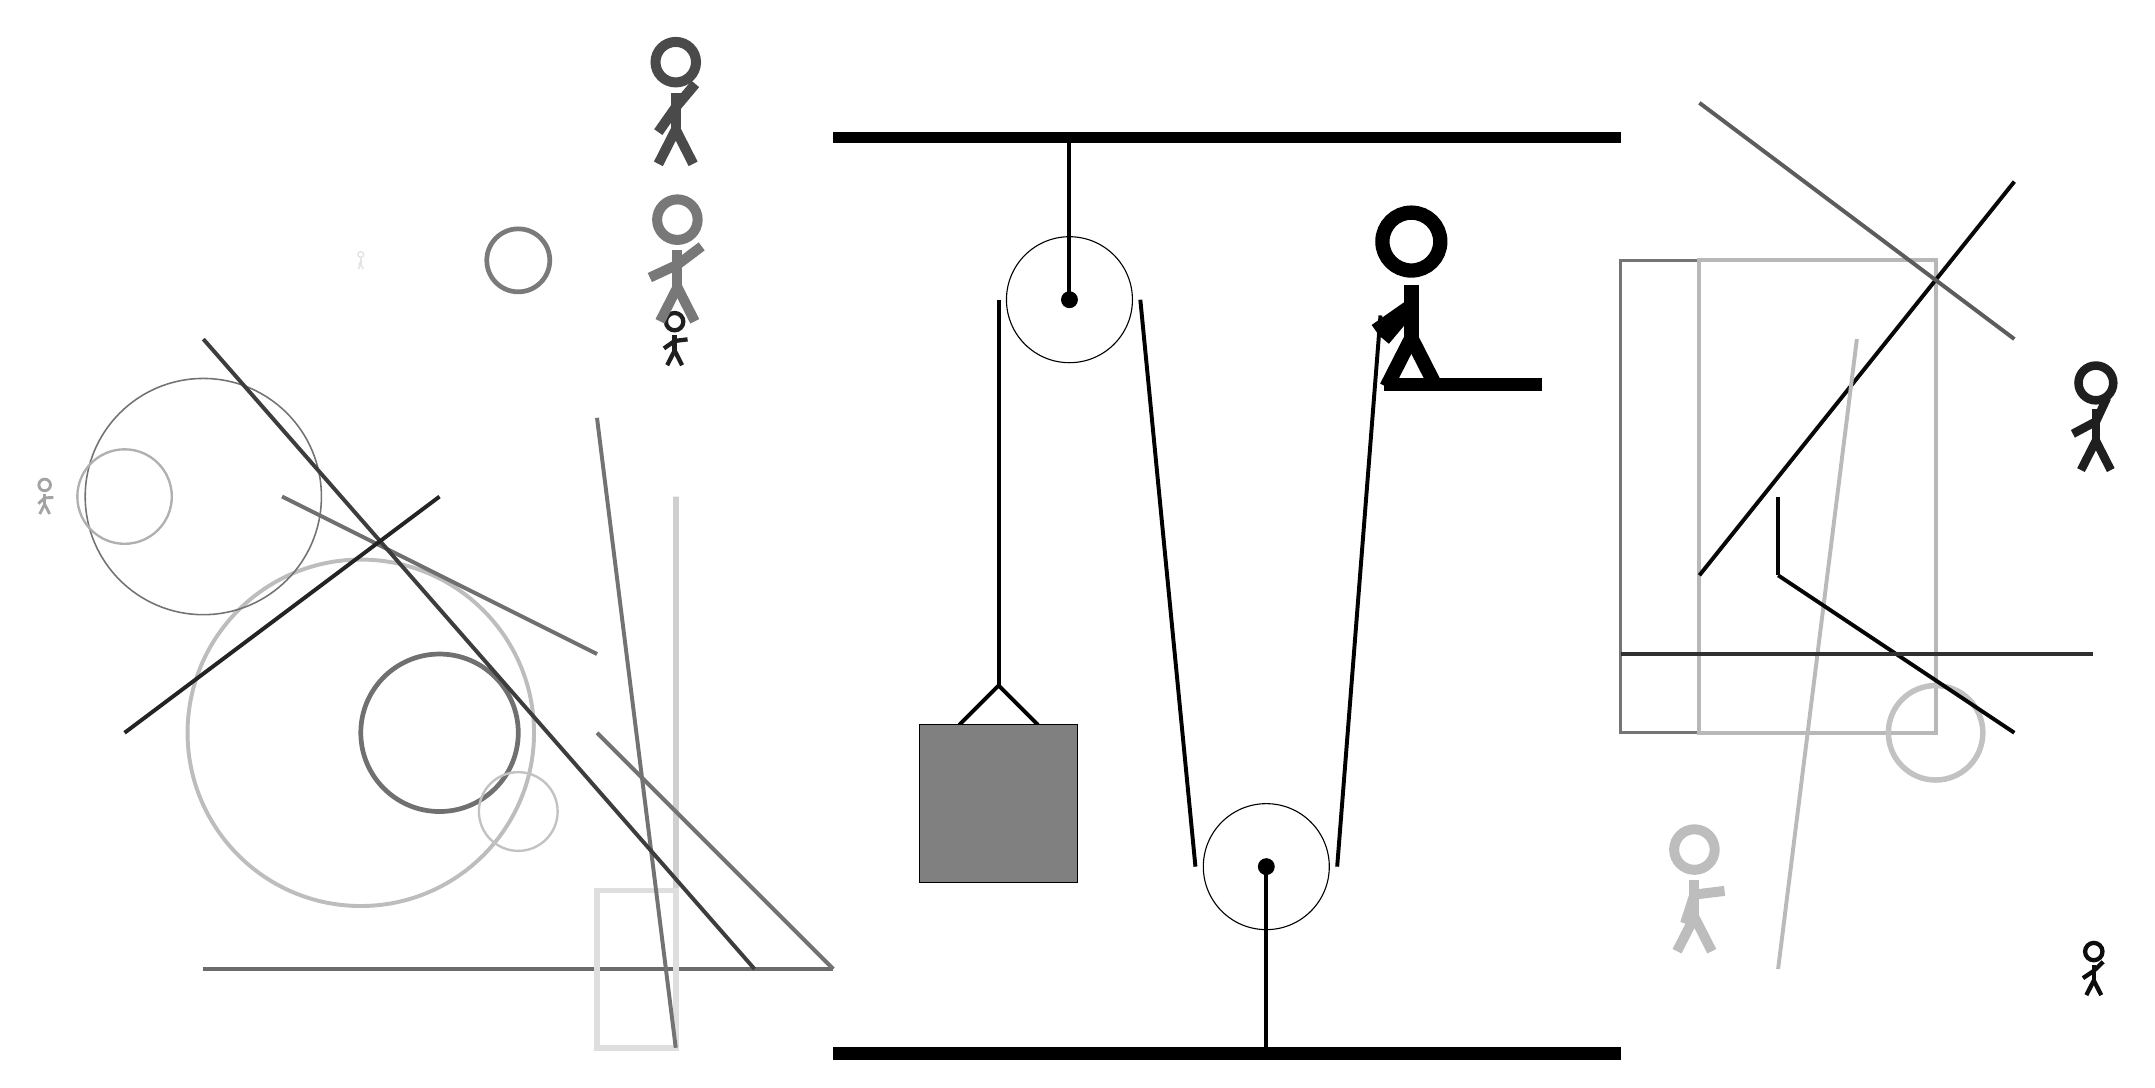
\begin{tikzpicture}
			%%%%% START %%%%%
			
			\draw[fill=black] (-2, 11.5) rectangle (8, 11.625);
			
			\draw (3.5, 2.3) circle (0.8);
			\draw[fill=black] (3.5, 2.3) circle (0.1);
			\draw[line width=0.5mm] (3.5, 2.3) -- (3.5, 0);
			
			\draw (1, 9.5) circle (0.8);
			\draw[fill=black] (1, 9.5) circle (0.1);
			\draw[line width=0.5mm] (1, 11.5) -- (1, 9.5);
			
			\node[line width=0.5mm, color=black!88] at (-4, 9) {\Strichmaxerl[3][35][7]};
			
			\draw[line width=0.7mm, color=black!19] (-4, 0) rectangle (-4, 7);
			\draw[line width=0.4mm, color=black!54] (8, 4) rectangle (9, 10);
			\draw [line width=0.6mm, color=black!56](-7, 4) circle (1.0);
			\draw[line width=0.5mm, color=black!98](10, 7) -- (10, 6);
			\node[line width=0.5mm, color=black!95] at (14, 1) {\Strichmaxerl[3][34][44]};
			\node[line width=0.2mm, color=black!36] at (-12, 7) {\Strichmaxerl[2][43][2]};
			\draw[line width=0.5mm, color=black!58](-2, 1) -- (-10, 1);
			\node[line width=0.6mm, color=black!88] at (14, 8) {\Strichmaxerl[6][28][65]};
			
			\node[line width=0.2mm, color=black!26] at (9, 2) {\Strichmaxerl[7][72][7]};
			\draw [line width=0.5mm, color=black!26](-8, 4) circle (2.2);
			\draw[line width=0.5mm, color=black!28] (9, 4) rectangle (12, 10);
			\draw[line width=0.5mm, color=black!97](13, 11) -- (9, 6);
			
			\node[line width=0.5mm, color=black!53] at (-4, 10) {\Strichmaxerl[7][25][37]};
			\draw [line width=0.7mm, color=black!24](12, 4) circle (0.6);
			\draw[line width=0.5mm, color=black!64](9, 12) -- (13, 9);
			
			\draw[line width=0.5mm, color=black!27](11, 9) -- (10, 1);
			\draw[line width=0.5mm, color=black!98](13, 4) -- (10, 6);
			\draw[line width=0.5mm, color=black!81](8, 5) -- (14, 5);
			\draw [line width=0.3mm, color=black!24](-6, 3) circle (0.5);
			\draw[line width=0.7mm, color=black!13] (-4, 0) rectangle (-5, 2);
			
			\draw [line width=0.2mm, color=black!55](-10, 7) circle (1.5);
			\node[line width=0.7mm, color=black!11] at (-8, 10) {\Strichmaxerl[1][61][86]};
			\node[line width=0.3mm, color=black!71] at (-4, 12) {\Strichmaxerl[7][55][50]};
			\draw [line width=0.6mm, color=black!52](-6, 10) circle (0.4);
			
			\draw[line width=0.5mm, color=black!55](-5, 8) -- (-4, 0);
			
			\draw[line width=0.5mm, color=black!56](-5, 5) -- (-9, 7);
			\draw[line width=0.5mm, color=black!55](-5, 4) -- (-2, 1);
			\draw[line width=0.5mm, color=black!76](-3, 1) -- (-10, 9);
			
			\draw [line width=0.3mm, color=black!31](-11, 7) circle (0.6);
			\draw[line width=0.5mm, color=black!86](-7, 7) -- (-11, 4);
			
			
			\draw[line width=0.5mm](-0.4, 4.1) --  (0.1, 4.6) -- (0.6, 4.1);
			\draw[fill=black!50] (-0.9, 4.1) rectangle (1.1, 2.1);
			
			\draw[line width=0.5mm](0.1, 9.5) -- (0.1, 4.6);
			\centerarc[line width=0.5mm](1, 9.5)(180:0:0.9)
			\draw[line width=0.5mm](1.9, 9.5) -- (2.6, 2.3);
			\centerarc[line width=0.5mm](3.5, 2.3)(180:360:0.9)
			\draw[line width=0.5mm](4.4, 2.3) -- (4.95, 9.3);
			
			\node at (5.3, 9.5) {\Strichmaxerl[10][35][-130]};
			\draw[fill=black] (5, 8.5) rectangle (7, 8.35);
			
			\draw[fill=black] (-2, 0) rectangle (8, -0.15);
			
			%%%%% END %%%%%
		\end{tikzpicture}
	\end{figure}	
\end{document}